\section{Error Quantification \&  Cutoff Frequency Variations}

The cutoff frequency was then varied within a frequency range of $10^{-2}$ to $10^2$ $\frac{rad}{s}$ and the above statistics were generated for all of them as described in Appendix \ref{sec:cutoff_error_variation_code}. With the aim of characterizing the error of each sensor output, the statistical analysis was mainly interested in seeing the point where the full system signal error is minimal. However, varying the simulation time changed this optimal value. Hence, futher analysis was done to practically determine the practical optimal cutoff frequency.

Since multidimensional data needed to be analysed, the Pandas Python data science package was used alongside Matplotlib 3D. Note that within the following analysis, exact values are always given since the random noise inputted in each heading signal simulation changes does not provide an identical response, but overall value ranges are noticed. This was done for the accuracy of attempting a real world heading signal simulation.

The three main sensor outputs that vary with the cutoff frequency are the gyro filter, compass filter and full system accordingly. Figures \ref{fig:full_system_cutoff_frequency} to \ref{fig:compass_filter_error_cutoff_frequency} describe provide a 3D plot representing how the time response and respective errors change with the variation of cutoff frequency. Whilst making the figures, a small section of the varied cutoff frequencies was selected to specifically demonstrate the changing behaviour. Figure \ref{fig:full_system_cutoff_frequency} shows how the overall time response of the full system varies. Within the range of 0 to 1.75 $rad/s$, it can be observed how response oscillations increase by comparing the initial amplitude of the time response to the final amplitude. To visualize this clearer, Figure \ref{fig:full_system_error_cutoff_frequency} demonstrates the difference between the full response and the input heading within a larger cutoff frequency range and the increase is noticeable. This is expected since it would mean that the compass, whose bode plot starts becoming nonlinear between 1 and 2 $rad/s$, begins responding to higher frequency oscillations.

% Full System vs Cutoff Frequency
\begin{figure}[H]
\centering
\begin{subfigure}{0.5\linewidth}
  \centering
  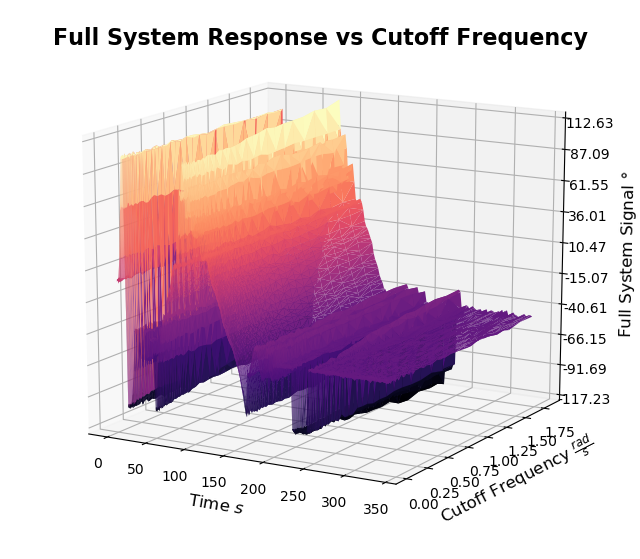
\includegraphics[width=\linewidth]{img/fullSystemCutoffFrequency.png}
  \caption{Full system amplitude time response vs cutoff frequency.}
  \label{fig:full_system_cutoff_frequency}
\end{subfigure}%
\begin{subfigure}{0.5\linewidth}
  \centering
  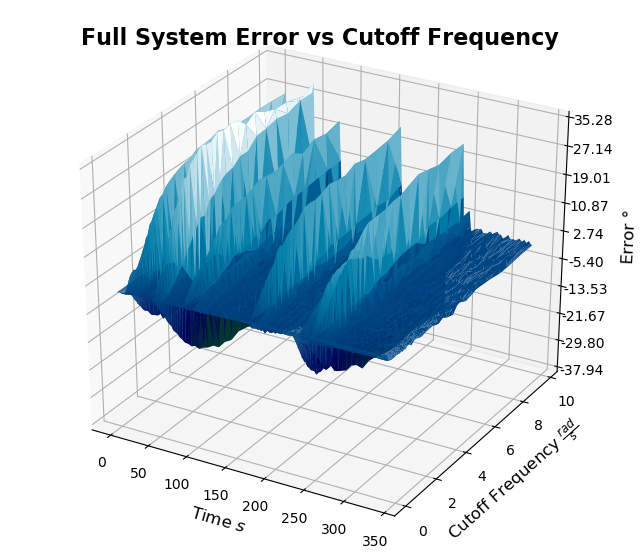
\includegraphics[width=\linewidth]{img/fullSystemErrorCutoffFrequency.png}
  \caption{Full system error variation in time}
  \label{fig:sub2}
\end{subfigure}
\caption{Full system error time response vs cutoff frequency. Note the difference in scales to adequately represent changes.}
\label{fig:full_system_error_cutoff_frequency}
\end{figure}

Figure \ref{fig:gyro_filter_error_cutoff_frequency} also demonstrates an interesting behaviour within a small cutoff frequency range of 0 to 1.75 $rad/s$. The gyro filter error response magnitude reaches steady state from 1.75 $rad/s$ to the rest of the cutoff frequencies, which is why only this range was modelled. The transient variation of the magnitude of the error in this graph within 0 and 1.25 $rad/s$ could be considered as differential change due to cutoff frequency change in the form $\frac{d(GyroEror)}{d(CutoffFrequency)}$. The steady state value is reached around 1 $rad/s$, and from this point on-wards the $\frac{d(GyroEror)}{d(CutoffFrequency)} \approx 0$. Considering this as a uni-variate optimization problem, it could be said that this is the optimal cutoff point since the compass is designed to operate adequately at lower frequencies. Also observing Figure \ref{fig:compass_filter_error_cutoff_frequency}, a 1 $rad/s$ compass cutoff frequency has relatively low error values in comparison to the rest of its error magnitude response after exponentially decreasing from a maximum near 0 $rad/s$. Hence, even in 3D space, the behaviour of complementary filter errors are demonstrated also when steady state values are reached. However, to fully discuss this, statistical time domain analysis needs to be performed.

% Gyro  and Compass Cutoff Filters over time
\begin{figure}[H]
\centering
\begin{subfigure}{0.5\linewidth}
  \centering
  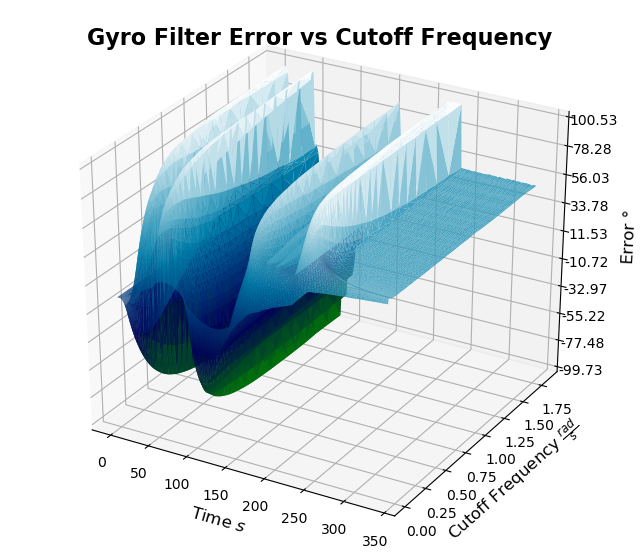
\includegraphics[width=\linewidth]{img/gyroFilterErrorCutoffFrequency.png}
  \caption{Gyro filter error variation with cutoff frequency over time.}
  \label{fig:gyro_filter_error_cutoff_frequency}
\end{subfigure}%
\begin{subfigure}{0.5\linewidth}
  \centering
  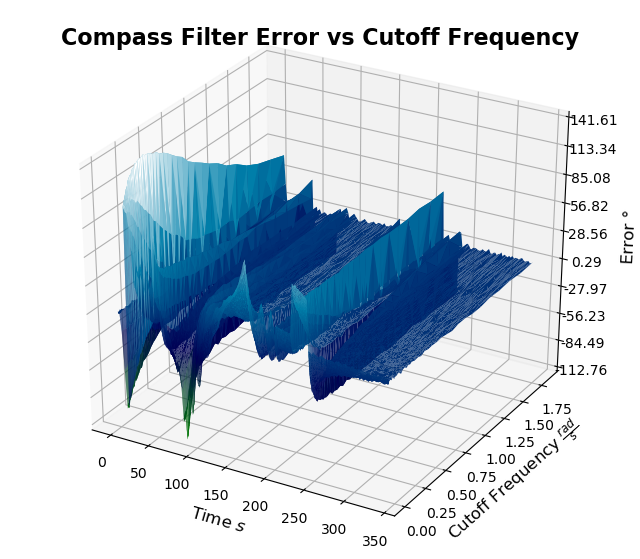
\includegraphics[width=\linewidth]{img/compassFilterErrorCutoffFrequency.png}
  \caption{Compass filter error variation with cutoff frequency over time.}
  \label{fig:sub2}
\end{subfigure}
\caption{Compass filter error variation with cutoff frequency over time.}
\label{fig:compass_filter_error_cutoff_frequency}
\end{figure}

% Carque et al. \cite{carque2011sensor} and Pasocal et al. \cite{pascoal2000navigation} demonstrate the accuracy benefits of sensor fusion
% ➢ T5.4 Propose a metric and quantify the error for each sensor output and for the fused output over the whole simulated flight. Hint – you may want to review the time domain statistical measures lecture. (10 marks)
A statistical metric cannot be chosen at random to quantify this error since all metrics provide different information about the signal data distribution. A comprehensive overall error metric might be a combination of different data statistics. In order to adequately select the error metric, or combined error metric, the following analysis were performed for both the raw signals and error sets: maximum, minimum, mean, standard deviation, variance, skewness, kurtosis, moments from 1 to 4, RMS, and 3dB power bandwidth (not for errors).  

Figures \ref{fig:sample_statistical_metrics} provides a sample of statistical metrics for all the signal errors whilst changing the cutoff frequency. In order to minimize the magnitude of the full system error, ideally its magnitude should be regularly near zero. However, realistically, because the incremental zero offset errors introduced into the gyro compass design that cannot be corrected via frequency filtering, the ideal value of the full system is when it matches the gyro system offset error within this model. It was noted that by varying the simulation time, the time-domain statistical optimal parameters vary; given the larger effect of the gyro system offset error. Hence, even if the time domain statistical parameters varied, what is required is selecting a cutoff frequency that is in steady state of the slope $\frac{d(SignalResponse)}{d(cutoffFrequency)} = 0$. At that point, the compass filter output is still at its maximum and the gyro filter output will have its standard zero-offset expected error. Hence, the response of the compass filters is not minimized specially when this is used to calibrate the gyro in flight during steady conditions. However, further time-domain statistical analysis will be performed in order to compare the optimal low statistic points for a specific simulation flight length with the steady cutoff frequency that is independent of this. This is because whilst the error magnitude may increase the overall zero offset rate is constant since it is not coupled mathematically as a function of the change of the cutoff frequency seen in Figure \ref{fig:full_system_error_cutoff_frequency}, only the filters are. 

The effect of varying cutoff frequencies on the amplitude of the response can be primarily observed in Figures \ref{fig:error_min} and \ref{fig:error_max}. If the cutoff frequency induces more oscillations, this will lead to larger differences within the response. It can be observed between the $10^{1}$ to $10^{2}$ regions that the full system response error stabilizes at a minima of around -60 and maxima of around 80. By the shape of the graphs, it can be inferred that oscillations differences are larger when the cutoff frequency is larger. This is expected since the compass filter would mainly respond to most flight oscillations, despite being optimized for lower frequencies.

The first aspect that will be analysed from the error differences are the standardized data moments which basically identify the crucial peak points within the data.

The mean ($\propto 1^{st} Moment$) is ${\rm}\mu ={\frac {1}{N}}\sum _{i=1}^{N}x_{i}.$ where $N$ is the time domain signal magnitude sample points. The mean is represented in Figure \ref{fig:error_mean}, but does not fully account for transient responses. However, it provides a general indication that the overall response averaged error $\frac{d(FullSystemEror)}{d(CutoffFrequency)}$ stabilizes to 0.1$\degree$ at a 0.13 $rad/s$. However, the mean has already reached a near zero value before the $10^{-1}$. Potentially because the system has not run for long enough, the mean is near 0 and has not stabilized yet to the gyro system error. It is also worth noting that there is a near-inflection point for both the compass (blue) and gyro (green) filter error plots at this point, which is related to a cutoff frequency change. Hence, the mean might not be an accurate error metric for the overall system error minimization response. % todo assume first moment

The standard deviation ($\propto 2^{nd} Moment$) for each cutoff frequency is $\sigma ={\sqrt {{\frac {1}{N}}\sum _{i=1}^{N}(x_{i}-\mu )^{2}}}$ where $X_i$ is a time domain sample point, and this illustrates how large the distribution of overall errors is from the averaged value in Figure \ref{fig:error_standard_deviation}. Hence, for a larger $\sigma$ is, it means that $X_i$ varied errors can be drastically different from the overall averaged error. It could also mean that oscillations could be very large but quick. When the objective is to minimize both transient and overall errors, it is desired that the overall error magnitude value and distribution of errors to be near zero. The full system has an minimum point where the distribution is near 0 at 0.048 $rad/s$. Again there appears to be an inflection point at this value for the compass and gyro filters. However, since it is known that practically that minimum is not the ideal value due to the increasing zero-offset observed during large simulation times, it can also be observed that at about 1 $rad/s$ the gyro filter error and compass filter errors reach a steady state value. The full system plot intersects also with the gyro system error plot. This was expected from observing their time responses in Figure \ref{fig:compass_filter_error_cutoff_frequency}.

Again regarding the full system signal, the skewness ($\propto 3^{nd} Moment$) and kurtosis ($\propto 4^{th} Moment$) in Figures \ref{fig:error_skewness} \& \ref{fig:error_kurtosis}  provide understanding of the asymmetrical accentuation of the probabilistic distribution of data around a overall mean value. The interesting aspect is that both signals have a maximum at the values around 0.048 $rad/s$. They also seem to reach steady state values slightly before or after $10^1$ $rad/s$ as expected from previous moments.

When characterizing the gyro system error, it is known that there will be zero offset as mechanical forces destabilize it during the heading flight. At its latest position, it has a $8.66 \degree$ difference for 350s heading flight. Assuming a linear slope, this offset error will only increase with longer flights, its slope in this simulation is $\approx 0.025 \degree/s = \approx 1.5 \degree/min$ as seen in Figure \ref{fig:raw_time_signals_full} which validates our design goal. Its standard deviation remains constant around 2.13 since the only changes are from a few high frequency turning rates that lead to higher errors (as observed) in Figure \ref{fig:raw_time_errors_full}.

The root mean squared RMS of a function $g(t)$ is ${\displaystyle g_{\text{RMS}}=\lim _{T\rightarrow \infty }{\sqrt {{1 \over {T}}{\int _{0}^{T}{[g(t)]}^{2}\,dt}}}.}$ where $T$ is the number of sample points of the response function $g(t)$. Because the mean of all the squared magnitudes of the signal are considered, it provides a general indication of the ``energy" value of the wave. It can also be noted that there is a minima around 0.048 $rad/s$. This full system error has an inflection point around 1 $rad/s$ where it intersects with the gyro system error probably due to the inverse stabilization of the the gyro and compass filter magnitudes.

Hence, an error metric for each sensor is required to be derived. It is known that the RMS and standard deviation are the most accurate statistics to determine the optimal cutoff frequency at the intersection of the gyro system error and the full system error. The error with any other cut-off frequency can be determined by the absolute difference between the full system error and gyro system error accordingly. Also, because the gyro filter and compass filter behave nearly inversely, as in Figure \ref{fig:error_standard_deviation}, the difference between the two can be compared to an optimal difference in magnitude of 32.52 for the standard deviation and 37.63 for the RMS. Since there is an inflection point for both error signals, this can be related to the ideal minimum for that specific flight time and this point will move towards the right as the flight time is increased. Hence, a geometrical relationship can be derived from these graphs. Integrating this analysis together constraining it to give a value between 0 and unity of error can be written in Equation \ref{eq:error_metic}, where $E_m$ is the error metric, $\Delta\sigma$ is the difference in the standard deviation for that cut-off frequency $w_c$, and $\Delta\kappa$ is the difference in RMS values. The closer it is to 0, the cutoff frequency is closer to the ideal one.

\begin{equation}
    E_m(w_c) = \frac{32.52\Delta\Sigma}{37.63} + \frac{37.63 \Delta\kappa}{32.52}
    \label{eq:error_metic}
\end{equation}

This metric can be compared to different heading flights and possibly the ideal difference values can be calibrated after testing over a further range of frequencies and simulation time. In summary, multi-dimensional Big Data time statistical analysis was used to determine the optimal design parameters of a sensor fusion system.

\begin{figure}[H]
 % First
\begin{subfigure}{.5\textwidth}
  \centering
  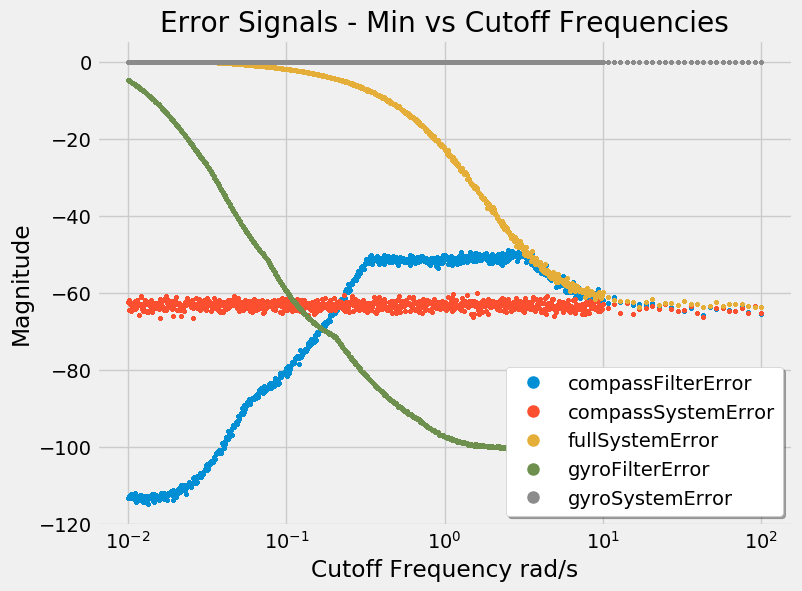
\includegraphics[width=\linewidth, height=\paperheight/5]{img/iterable/errorsSignals/errorminSignals.png}  
  \caption{Signal errors minimum value.}
  \label{fig:error_min}
\end{subfigure}
% Second
\begin{subfigure}{.5\textwidth}
  \centering
  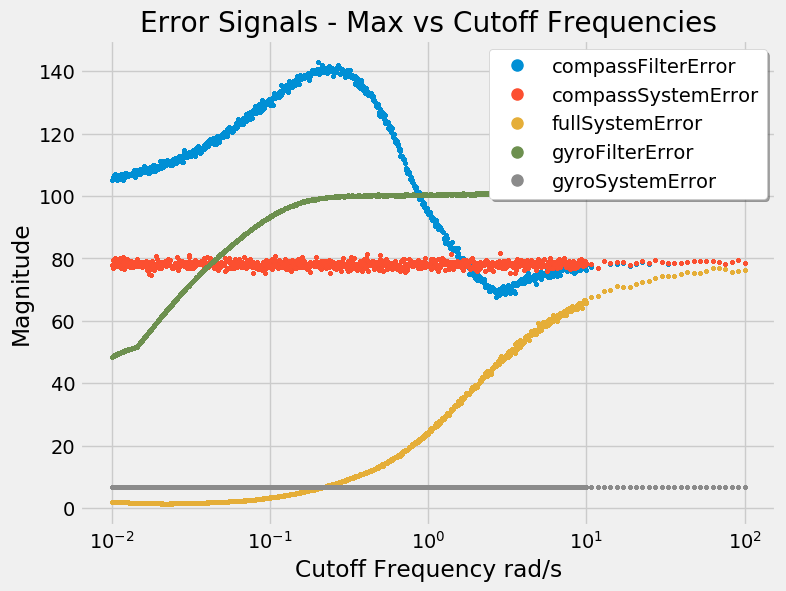
\includegraphics[width=\linewidth, height=\paperheight/5]{img/iterable/errorsSignals/errormaxSignals.png} 
  \caption{Signal errors maximum value.}
  \label{fig:error_max}
\end{subfigure}
% Third
\begin{subfigure}{.5\textwidth}
\centering
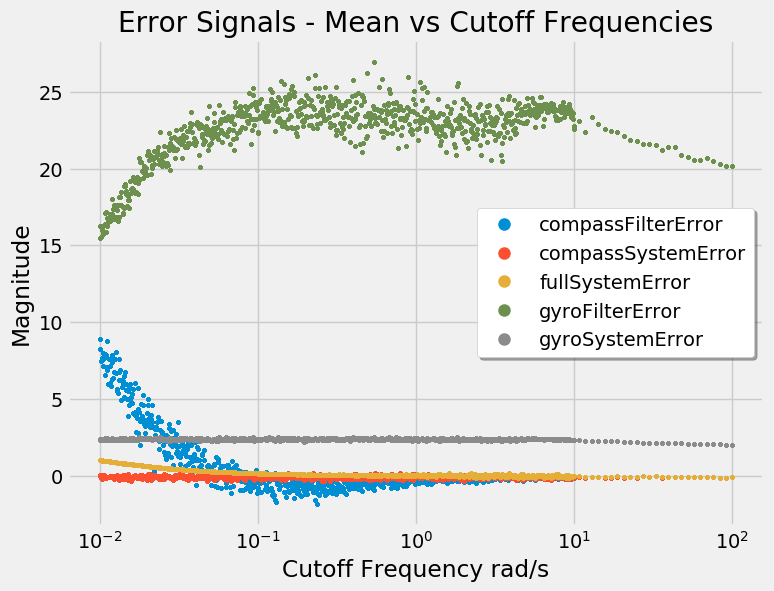
\includegraphics[width=\linewidth, height=\paperheight/5]{img/iterable/errorsSignals/errormeanSignals.png}  
  \caption{Signal errors mean value ($\propto1^{st}$ Moment)}
\label{fig:error_mean}
\end{subfigure}
  % Fourth
\begin{subfigure}{.5\textwidth}
  \centering
  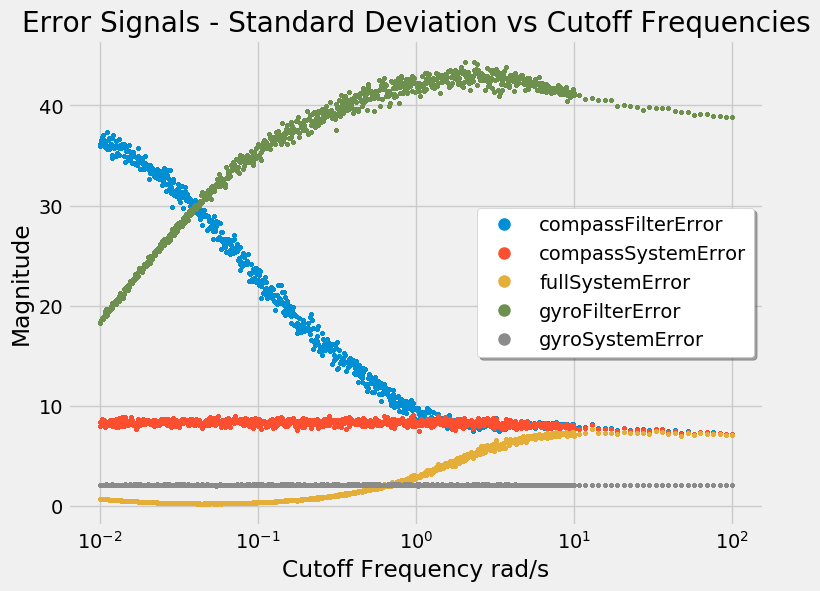
\includegraphics[width=\linewidth, height=\paperheight/5]{img/iterable/errorsSignals/errorstandardDeviationSignals.png}  
  \caption{Signal errors standard deviation. ($\propto2^{nd}$ Moment)}
  \label{fig:error_standard_deviation}
\end{subfigure}
% Fifth
\begin{subfigure}{.5\textwidth}
  \centering
  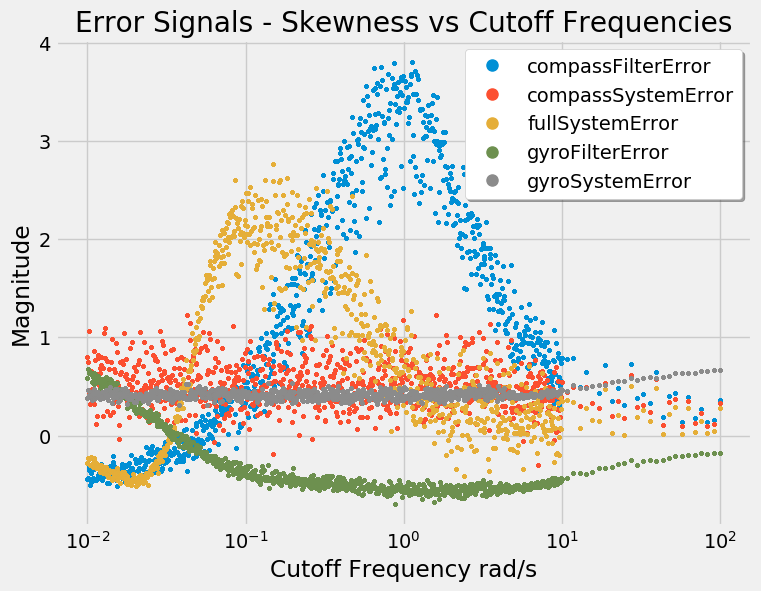
\includegraphics[width=\linewidth, height=\paperheight/5]{img/iterable/errorsSignals/errorskewnessSignals.png}  
  \caption{Signal errors skewness. ($\propto3^{rd}$ Moment)}
  \label{fig:error_skewness}
\end{subfigure}
  % Sixth
\begin{subfigure}{.5\textwidth}
  \centering
  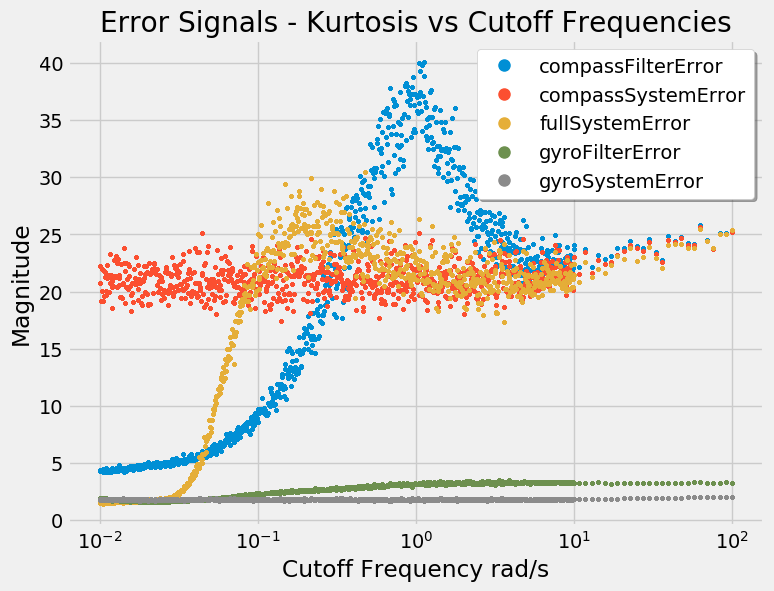
\includegraphics[width=\linewidth, height=\paperheight/5]{img/iterable/errorsSignals/errorkurtosisSignals.png}  
  \caption{Signal errors kurtosis ($\propto4^{th}$ Moment)}
  \label{fig:error_kurtosis}
\end{subfigure}
% Seventh
\begin{subfigure}{.5\textwidth}
  \centering
  % Eigth
  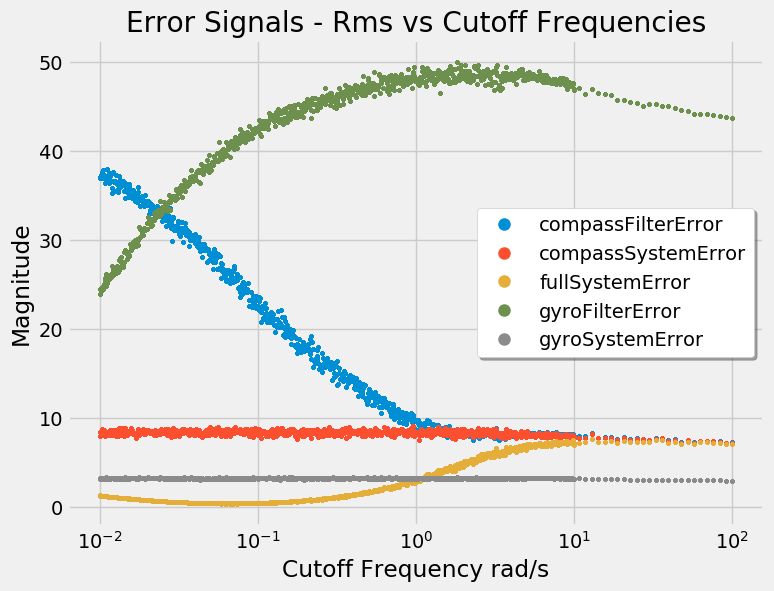
\includegraphics[width=\linewidth, height=\paperheight/5]{img/iterable/errorsSignals/errorrmsSignals.png}  
  \caption{Signal error RMS (Energy).}
  \label{fig:error_rms}
\end{subfigure}
\caption{Error differences with cutoff frequencies}
\label{fig:sample_statistical_metrics}
\end{figure}




% https://tex.stackexchange.com/questions/53458/inserting-figures-using-loops

% \section{Cutoff Frequency Variations}
% ➢ T5.5 Explore how variations in the True Heading Signal or in the filter cut-off frequency affect the measured error. (10 marks) 